\capitulo{4}{Técnicas y herramientas}

\section{Angular}\label{angular}
Angular es un framework de desarrollo de aplicaciones web que es de código abierto y está mantenido por Google, está basado en TypeScript, que es similar a JavaScript y aporta un tipado estático y unas características avanzadas de ES6+, que mejoran la escalabilidad y la capacidad de mantenimiento de los proyectos. 

\begin{center}
  
\includegraphics[width=0.3\textwidth]{img/angular-logo.png}\\
  \small Logotipo de Angular
\end{center}

El principal núcleo que diferencia y da ventaja a Angular respecto a otros frameworks es el concepto de componentes, que son unidades que combinan html, typescript y css. Cada componente representa una de las partes que se ven en la interfaz de usuario y se pueden anidar unos con otros formando jerarquías que definirán la estructura final que tendrá la aplicación. Estos componentes se agrupan en modulos, que permiten organizar el código en diferentes funcionalidades y admitir de esa forma la carga perezosa (lazy loading) para que se cargue solo la informacion esencial en cada ventana y se mejore el rendimiento.

Para hacer la gestión de la comunicación entre componentes y servicios, Angular tiene un sistema que se llama inyección de depencencias, con el que se registran en los injectors o contenedores los servicios que sirven para acceder a datos.

Angular también incluye un enrutador (Router) que permite definir rutas y navegacion dentro de la aplicacion web, gestionando los parámetros, posibles rutas hijas y los guards que controlan el acceso a apartados de la aplicacion segun los permisos que se quieran dar. Junto con angular cli, ofrece un ecosistema muy maduro. lo que lo convierte en una opción sólida para construir aplicaciones web robustas, mantenibles y de gran escala.

\section{Angular CLI}\label{angular-cli}
Es una herramienta de línea de comandos que acelera la creación, compilación y el despliegue de los proyectos, de manera que permite aplicar mejores prácticas de forma automática.

\begin{center}
  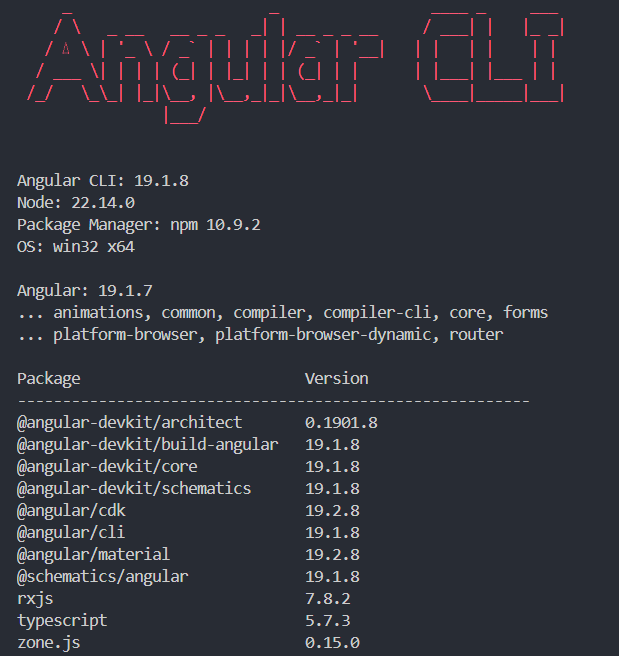
\includegraphics[width=0.7\textwidth]{img/angular-cli.png}\\
  \small Angular CLI
\end{center}

\section{TypeScript}\label{typescript}
TypeScript es un superset tipado de JavaScript que está desarrollado por Microsoft, lo que indica que todo el código JavaScript válido también lo es en TypeScript, pero con algunas capacidades añadidas como la declaración de tipos estáticos. Está diseñado para desarrollar aplicaciones grandes y capaz de detectar errores a la hora de compilar y evitar problemas.

Con la declaración de tipos estáticos se define una diferencia importante con JavaScript, ya que permite tipificar y que el lenguaje usado sea fuertemente tipado.

\subsection{Ventajas de TypeScript}

\begin{itemize}
  \item \textbf{Buen mantenimiento y escalabilidad}:
        Para proyectos grandes, los tipos ofrecen una red de seguridad que permite evitar errores y facilita el entendimiento de interfaces y unión entre módulos.
  \item \textbf{Mejor experiencia de desarrollo}: 
        Los editores de código (IDEs) pueden ofrecer autocompletado, navegación entre definiciones y verificación de errores gracias al análisis estático.
  \item \textbf{Características avanzadas}:
        Tiene genericos, decoradores y el sistema de tipos que evoluciona para cubrir patrones complejos.
\end{itemize}

\begin{center}
  
\includegraphics[width=0.25\textwidth]{img/typescript-logo.png}\\
  \small Logotipo de TypeScript
\end{center}


\section{HTML y CSS}\label{html-css}
Estos dos lenguajes de programación se utilizan en conjunto para crear la gran mayoría de páginas web.

\subsubsection{HTML}

HTML (HyperText Markup Language) es un lenguaje de marcado basado en etiquetas que define la parte del contenido que se va a mostrar en una web. Cada elemento como encabezados (\texttt{<h1>–<h6>}), párrafos (\texttt{<p>}), enlaces (\texttt{<a>}) o listas (\texttt{<ul>}, \texttt{<ol>}) se escribe con una etiqueta para abrir y cerrar.

\begin{center}
  
\includegraphics[width=0.2\textwidth]{img/html-logo.png}\\
  \small Logotipo de HTML
\end{center}

\subsubsection{CSS}

CSS (Cascading Style Sheets) es un lenguaje de hojas de estilo que indica cómo se deben mostrar los elementos del HTML. A través de selectores y propiedades (por ejemplo, \texttt{color}, \texttt{font-size}, \texttt{margin} o \texttt{display}), CSS permite mantener separados el contenido y su estilo, facilita el mantenimiento y mejora del diseño y permite adaptar la interfaz de usuario a diferentes tamaños de pantalla con técnicas responsive.

\begin{center}
  
\includegraphics[width=0.15\textwidth]{img/css-logo.png}\\
  \small Logotipo de CSS
\end{center}


\section{.NET para APIs}\label{net}

.NET, a través de ASP .NET Core, ofrece un framework que es ligero y modular y además está especialmente optimizado para construir APIs RESTful con un alto rendimiento y buena escalabilidad. Su modelo de programación está basado en controladores (\texttt{Controllers}), rutas y servicios.

\begin{itemize} 
  \item \textbf{Documentación automática con Swagger}: integración de forma nativa con \texttt{Swashbuckle.AspNetCore} para generar especificaciones OpenAPI y poder exponer Swagger UI sin tener que crear código adicional.  
  \item \textbf{Entity Framework Core}: ORM (Object-Relational Mapping o Mapeo Objeto-Relacional) ligero y extensible para mapear modelos a bases de datos relacionales, con soporte para migraciones, consultas y seguimiento de cambios.  
  \item \textbf{Seguridad y validación}: tiene soporte para autenticar las APIs basada en tokens como pueden ser JWT y OAuth2.  
\end{itemize}

 
\begin{center}
  
\includegraphics[width=0.25\textwidth]{img/net-logo.png}\\
  \small Logotipo de .NET Core
\end{center}


\section{Visual Studio Code}\label{visual-studio-code}

Visual Studio Code (VS Code) es un editor de código gratuito y multiplataforma que está desarrollado por Microsoft. Combina la ligereza y rapidez con funcionalidades avanzadas típicas de un IDE (entorno de desarrollo integrado), ofreciendo un consumo de recursos moderado en distintas plataformas. Visual Studio Code se centra en mejorar la productividad del desarrollador mediante una interfaz intuitiva y un sistema de pestañas que permite navegar entre ficheros facilmente.

Entre sus características más destacadas están:
\begin{itemize}
  \item \textbf{IntelliSense}: sugerencias de código inteligentes y autocompletado, permitiendo una experiencia mejor y una agilidad mayor. 
  \item \textbf{Depuración integrada}: permite poner puntos de interrupción, inspeccionar variables saltar paso a paso y tiene una consola de depuración unificada.
  \item \textbf{Terminal integrado}: proporciona acceso directo a la línea de comandos dentro del propio editor, permitiendo ejecutar comandos sin tener que salir del editor.  
  \item \textbf{Control de versiones Git}: tiene un panel que enseña las diferencias, historial de commits, ramas y etiquetas y tiene botones para realizar acciones rápidas para commit, push, pull y resolución de conflictos.  
  \item \textbf{Extensiones y Marketplace}: ofrece muchas extensiones para diferentes lenguajes, temas de estilo, depuradores y distintas utilidades.  
  \item \textbf{Workspaces y configuración}: el espacio de trabajo está separado por carpetas y tiene una interfaz que permite la navegación sencilla por ellas.  
\end{itemize}

Este ha sido el editor que he usado para desarrollar la parte del front hecho con Angular, por todas estas ventajas que tiene y sobretodo por las facilidades y comodidades que aportan las extensiones.

\begin{center}
  
\includegraphics[width=0.2\textwidth]{img/vscode-logo.png}\\
  \small Logotipo de Visual Studio Code
\end{center}


\section{Visual Studio 2022}\label{visual-studio}

Visual Studio 2022 es un entorno de desarrollo integrado (IDE) para Windows, está diseñado para dar soporte a proyectos de gran tamaño y múltiples lenguajes. Este entorno, aprovecha más memoria y potencia de CPU, lo que se traduce en tiempos de carga más rápidos, soluciones con muchos archivos y depuración fluida sin necesidad de subdividir proyectos.

Entre sus características más relevantes están:
\begin{itemize}
  \item \textbf{Plantillas de API ASP.NET Core}: permite crear proyectos Web API con un solo click, incluyendo la estructura de los controladores, archivos \texttt{Program.cs} y \texttt{launchSettings.json} preconfigurados para ejecutar en IIS Express.
  \item \textbf{Integración nativa con Swagger}: una de las características interesantes es que añade y configura \texttt{Swashbuckle.AspNetCore} directamente desde el asistente de NuGet, que genera automáticamente especificaciones OpenAPI y expone Swagger UI para probar los endpoints que se van creando.
  \item \textbf{IntelliSense y refactorización para C\#}: implementa una herramienta que ayuda a completar el código de forma inteligente y con sugerencias basadas en patrones de uso de .NET, que facilitan la creación de controladores, modelos y servicios con interfaces fuertemente tipadas.
  \item \textbf{Extensibilidad y extensiones .NET}: permite instalar extensiones como Pomelo Entity o Entity Framework Tools para extender capacidades de los proyectos de API sin salir del IDE.
\end{itemize}

\begin{center}
  
\includegraphics[width=0.2\textwidth]{img/visualstudio-logo.png}\\
  \small Logotipo de Visual Studio Code
\end{center}


\section{Swagger}\label{swagger}

Swagger es un conjunto de herramientas que están basadas en la especificación de OpenAPI que permite diseñar, documentar y probar las APIs de forma automática. En el ecosistema .NET, su integración se realiza habitualmente mediante el paquete NuGet \texttt{Swashbuckle.AspNetCore}, lo que ofrece:

\textbf{Interfaz interactiva (Swagger UI)}: expone una web donde se pueden explorar y ejecutar todos los endpoints de la API sin herramientas externas.

\textbf{Validación y pruebas rápidas}: facilita la comprobación de respuestas y códigos de estado en tiempo real, acelerando el proceso de desarrollo y la detección de errores.


\section{LaTeX}

LaTeX es un sistema de preparación de documentos que está basado en el lenguaje TeX, diseñado para producir documentos una buena calidad. Es especialmente valorado en entornos más académicos y científicos debido a su capacidad para gestionar fácilmente fórmulas matemáticas complejas, bibliografías y diferentes idiomas.

\begin{center}
  
\includegraphics[width=0.3\textwidth]{img/latex-logo.png}\\
  \small Logotipo de LaTeX
\end{center}

\subsection{Overleaf}

Overleaf es un editor de LaTeX basado en la nube que ofrece un entorno colaborativo y accesible desde cualquier navegador. En el, integra un compilador en tiempo real, que permite hacer una vista previa del documento y tiene detección de errores, esto facilita el trabajo en equipo y la revisión en equipos de documentos académicos, artículos y tesis. Permite crear e iniciar proyectos sin tener la necesidad de instalar ningún software localmente y compartir fácilmente el resultado.

\begin{center}
  
\includegraphics[width=0.2\textwidth]{img/overleaf-logo.jpg}\\
  \small Logotipo de Overleaf
\end{center}

\section{Control de versiones}\label{control-versiones}
Git es un sistema de control de versiones distribuido que está diseñado para poder gestionar el historial de cambios en proyectos de software.
\href{https://git-scm.com/}{Git}

\begin{center}
  
\includegraphics[width=0.3\textwidth]{img/git-logo.png}\\
  \small Logotipo de Git
\end{center}


\section{Github}\label{github}
\href{https://github.com/}{Github} es una plataforma en la nube que permite subir proyectos de software que utilizan el sistema de control de versiones Git. 

\begin{center}
  
\includegraphics[width=0.2\textwidth]{img/github-logo.png}\\
  \small Logotipo de GitHub
\end{center}

Subir código a un repositorio de GitHub implica los siguientes pasos básicos:

\subsection{Inicializar o clonar un repositorio Git}
Dentro de la carpeta de un proyecto, permite crear un repositorio local.
Cuando hay un proyecto existente, permite clonarlo para traer una copia local.

\subsection{Gestionar cambios con commits}
Después de crear o modificar archivos, se añaden al área de preparación (staging area) y se registran los cambios con un commit.

\subsection{Conectar el repositorio local con GitHub}
Si no se ha clonado, se puede añadir una URL remota en la que subir el código.

\subsection{Enviar (push) cambios al repositorio en GitHub}
Para subir la rama principal

\subsection{Trabajo colaborativo y ramas}
Ramas (`branches`): consiste en crear nuevas líneas de desarrollo y cambiarse a ellas.
Pull requests (PR): en la interfaz web de GitHub, proponer que tu rama se fusione (“merge”) en la rama principal tras revisión de código.

\subsection{Beneficios de usar GitHub}
Historial de versiones: permite regresar a estados anteriores del proyecto.
Colaboración: múltiples desarrolladores pueden trabajar simultáneamente sin pisarse cambios.
Visibilidad: proyectos open-source se comparten con la comunidad; repositorios privados para código interno.

Con lo que, subir los códigos a GitHub no consiste solamente en copiar y pegar ficheros, sino en aprovechar todo un ecosistema de control de versiones, asegurando que cada cambio quede documentado, pueda revisarse y desplegarse siguiendo buenas prácticas de desarrollo.


\section{HeidiSQL con MySQL}\label{heidi-sql}
HeidiSQL es un cliente gráfico gratuito para Windows diseñado principalmente para gestionar bases de datos MySQL, MariaDB y otros motores compatibles (como por ejemplo PostgreSQL o Microsoft SQL Server). 

\begin{center}
  
\includegraphics[width=0.25\textwidth]{img/heidi-logo.png}\\
  \small Logotipo de HeidiSQL
\end{center}

Al usarlo con MySQL, HeidiSQL ofrece una interfaz intuitiva que permite:
Conectarse y navegar por servidores MySQL mediante un administrador de sesiones, donde puedes guardar múltiples configuraciones de conexión (host, puerto, usuario, contraseña, etc.).

Visualizar y editar estructuras de bases de datos, tablas, vistas y procedimientos almacenados con un explorador de objetos que muestra de forma jerárquica todos los elementos.
Ejecutar consultas SQL en un editor con resaltado de sintaxis, autocompletado y pestañas múltiples para trabajar en varios scripts a la vez.

Importar y exportar datos de forma sencilla: puedes volcar estructuras y datos a archivos SQL, CSV, XML o incluso sincronizar bases de datos entre servidores con su herramienta de comparación.

Monitorear la actividad del servidor MySQL (procesos activos, status variables) y obtener estadísticas básicas de rendimiento.

\begin{center}
  
\includegraphics[width=0.4\textwidth]{img/mysql-logo.png}\\
  \small Logotipo de MySQL
\end{center}

HeidiSQL es muy útil cuando se necesita un acceso rápido y eficiente a bases de datos MySQL sin complicaciones de configuraciones avanzadas ni licencias de pago.

\section{Google AI Studio e integración en .NET}\label{google-ai-studio}
Google AI Studio (antes conocido como Vertex AI Workbench) es la plataforma de Google Cloud que unifica herramientas para el desarrollo, entrenamiento, despliegue y monitorización de modelos de inteligencia artificial y machine learning. 

\begin{center}
  
\includegraphics[width=0.5\textwidth]{img/ai-studio-logo.png}\\
  \small Logotipo de Google AI Studio
\end{center}

\subsection{Integración con Google AI Studio en .NET}

La aplicación .NET se conecta a Google AI Studio empleando las librerías oficiales de Google Cloud para .NET, lo que permite aprovechar capacidades avanzadas de IA directamente desde nuestro entorno de desarrollo. El proceso de integración consta de cuatro pasos clave:

\begin{enumerate}
  \item \textbf{Instalación}: añadir el paquete NuGet  
    \texttt{Google.Cloud.AIPlatform.V1} al proyecto.
  \item \textbf{Autenticación}: configurar y utilizar una cuenta de servicio  
    cuyas credenciales se cargan en las variables de entorno.
  \item \textbf{Invocación de la API}: llamar a los métodos de la biblioteca  
    para entrenar, evaluar o desplegar modelos de Machine Learning.
  \item \textbf{Gestión y monitorización}: para procesar las respuestas de la API y supervisar métricas y registros desde el propio código .NET.
\end{enumerate}

Gracias a esta integración, se pueden automatizar tareas de aprendizaje automático sin abandonar todo el ecosistema de .NET, manteniendo una experiencia de desarrollo coherente.


\section{Herramientas integradas en Angular}

\subsection{Angular Animations}
Angular Animations es un módulo oficial que extiende la capacidad de Angular para crear transiciones y efectos dinámicos en la web. Mediante la API basada en funciones como \texttt{trigger}, \texttt{state} y \texttt{transition}, permite definir animaciones de entrada, de salida y cambios de estado en los componentes, además, garantiza un rendimiento bueno en los navegadores más usados actualmente.

\subsection{Angular Material}
Angular Material es la implementación de Material Design para Angular, tiene componentes que vienen preparados y listos para usar directamente como botones, tarjetas, diálogos, menús, tablas, etc. y utilidades del Angular CDK.

\subsection{Bootstrap}
Bootstrap es un framework CSS muy utilizado que, con bibliotecas como \texttt{ng-bootstrap} o \texttt{ngx-bootstrap}, se integra perfectamente en proyectos Angular. Esto proporciona un sistema con utilidades, estilos y componentes interactivos como modales, barras de navegación y botones, permitiendo acelerar el desarrollo de interfaces de usuario.

\subsection{Leaflet}
Leaflet es una librería JavaScript que sirve para tener en la web mapas interactivos, su integración en Angular se realiza con paquetes como \texttt{@asymmetrik/ngx-leaflet}. Tiene componentes y directivas que facilitan la creación de mapas, edición de mapas y permite poner punteros en los mapas (lo que se ha usado en este caso) para indicar lugares.

\subsection{Toastr}
Toastr es una librería que permite sacar notificaciones de tipo “toast” que, mediante el paquete \texttt{ngx-toastr}, se adapta para mostrar mensajes breves que salen para advertir de diferentes acciones. Permite configurar la posición, el tiempo que se muestran y los estilos de cada notificación a través de servicios, mejorando así la experiencia de usuario.

\subsection{FullCalendar}
FullCalendar es un plugin para añadir calendarios interactivos en la web. La integración con Angular se realiza a través de \texttt{@fullcalendar/angular}, que lo que hace es exponer componentes para renderizar vistas de meses, semanas o incluso días, permite gestionar eventos y personalizar la apariencia.


\section{Draw.io}\label{drawio}

Draw.io es una web gratuita que permite crear y editar diferentes gráficos como diagramas o flujogramas. 

Esta herramienta se usa para generar los diagramas que se muestran en la parte de los anexos.